\chapter{Final event selection and categorization}

%%%%%%%%%%%%%%%%%%%%%%%%%%%%%%%%%%%%%%%%%%%%%%%%%%%%%%%%%%%%%%
\section{Search for a WH resonance in the $\ell\Pgn\bbbar$ final state at $\sqrt{s}$ = 8 TeV}

%%%%%%%%%
\subsection{\ttbar background rejection}

%%%%%%%%%
\subsection{Final selection and control plots}

\begin{table}[htb]
\footnotesize
\begin{center}
\caption{Summary of final selection.}
\label{tab:cutsummaryWH}
\begin{tabular}{lcc}
\hline
\multicolumn{1}{c}{\textbf{Selection}} & \textbf{Value} & \textbf{Comments}\\
\hline
\multicolumn{1}{c}{\texttt{Tight} Lepton selection}\\
\cline{1-1}
Electron $\PT$ & $\PT > 90 \GeV$  & \\
Muon $\PT$ & $\PT > 50 \GeV$ & \\
Electron $\eta$ & $|\eta|_{\text{SC}} <2.5$ except [1.4442, 1.566] range & Avoid the ECAL gap.\\
Muon $\eta$  & $|\eta|<2.1$  & \\
\hline
\multicolumn{1}{c}{\texttt{Loose} Lepton selection}\\
\cline{1-1}
Electron $\PT$ & $\PT > 35 \GeV$ & \\
Muon $\PT$ & $\PT > 20 \GeV$ & \\
Electron $\eta$ & $|\eta|_{\text{SC}} <2.5$ except [1.4442, 1.566] range & Avoid the ECAL gap.\\
Muon $\eta$  & $|\eta|<2.4$ & \\
\hline
\multicolumn{1}{c}{CA8 jet selections}\\
\cline{1-1}
Jet $\PT$ &  $\PT >80~\GeV$ & Used for hadronic \\
Jet $\eta$  & $|\eta|<2.4$ except [1, 1.5] range & H reconstruction \\
\hline
\multicolumn{1}{c}{AK5 jet selections}\\
\cline{1-1}
Jet $\PT$ &  $\PT >30~\GeV$ & Used for b-veto \\
Jet $\eta$  & $|\eta|<2.4$ & jet selection\\
\hline
\multicolumn{1}{c}{\ETmiss selections}\\
\cline{1-1}
\ETmiss (electron ch.) &  \ETmiss$>80~\GeV$ & \\
\ETmiss (muon ch.) & \ETmiss$>40~\GeV$ & \\
\hline
\multicolumn{1}{c}{Boson selections}\\
\cline{1-1}
Pruned jet mass (signal)        & $ 110 < m_{jet}^{pruned} < 135 \GeV$ &  \\
Pruned jet mass (low-mass sideband)       & $ 40 < m_{jet}^{pruned} < 110 \GeV$ & \\
Pruned jet mass (high-mass sideband)     & $ 135 < m_{jet}^{pruned} < 150 \GeV$ & \\
Leptonic W $\PT$      &  $\PT > 200 \GeV$ & \\
Hadronic H $\PT$      &  $\PT > 200 \GeV$ & \\
Back-to-back topology & $\Delta R (\ell , H_{had}) > \pi/2$ $\,$ , $\,$  $\Delta \phi (H_{had} , \mbox{\ETmiss})>2$ & \\
                      & $\Delta \phi (H_{had} , W_{lep})>2$ & \\
B-tag veto      & no CSV Medium AK5 jet &  \\
		& within $\Delta R (ca8, ak5) = 0.8$ &  \\
Combined b-tagging cut	& $>= 2$ CSVL subjets if $\Delta R > 0.3$ of subjets & \\
			& $>= 1$ CSVL CA8 jet if $\Delta R < 0.3$ of subjets & \\ 
Top mass veto	& $ m_{top}^{leptonic} < 120 $ $||$ $ m_{top}^{leptonic} > 240 $ & \\
		& $ m_{top}^{hadronic} < 160 $ $||$ $ m_{top}^{hadronic} > 280 $ & \\
\hline
\multicolumn{1}{c}{Veto}\\
\cline{1-1}
Number of \texttt{loose} electrons & 0 & in addition to \texttt{tight} lepton \\
Number of \texttt{loose} muons & 0 & in addition to \texttt{tight} lepton \\
\end{tabular}
\end{center}
\end{table}

\begin{figure}[h!bp]
\centering
\begin{tabular}{lr}
\includegraphics[width=0.5\textwidth]{\cheight/WHanalysis/controlPlots/ele/can_h_ptlepton.pdf} &
\includegraphics[width=0.5\textwidth]{\cheight/WHanalysis/controlPlots/mu/can_h_ptlepton.pdf} \\
\includegraphics[width=0.5\textwidth]{\cheight/WHanalysis/controlPlots/ele/can_h_etalep.pdf} &
\includegraphics[width=0.5\textwidth]{\cheight/WHanalysis/controlPlots/mu/can_h_etalep.pdf} \\
\end{tabular}
\caption{ Lepton \pt and $\eta$ for electron channel (left) and muon channel (right) for events with $40 < m_{jet}^{pruned} < 110$ GeV. The signal is normalized to $0.1$ times of the selected events for the model considered (W', $M=1$ TeV).}
\label{fig:controlPlotsLepPtEta}
\end{figure}

\begin{figure}[h!bp]
\centering
\begin{tabular}{lr}
\includegraphics[width=0.5\textwidth]{\cheight/WHanalysis/controlPlots/ele/can_h_met.pdf} &
\includegraphics[width=0.5\textwidth]{\cheight/WHanalysis/controlPlots/mu/can_h_met.pdf} \\
\includegraphics[width=0.5\textwidth]{\cheight/WHanalysis/controlPlots/ele/can_h_pz_type2.pdf} &
\includegraphics[width=0.5\textwidth]{\cheight/WHanalysis/controlPlots/mu/can_h_pz_type2.pdf} \\
\end{tabular}
\caption{ \ETmiss and $pz_\nu$ (defined in Section) for electron channel (left) and muon channel (right) for events with $40 < m_{jet}^{pruned} < 110$ GeV. The signal is normalized to $0.1$ times of the selected events for the model considered (W', $M=1$ TeV).}
\label{fig:controlPlotsMETPz}
\end{figure}

\begin{figure}[h!bp]
\centering
\begin{tabular}{lr}
\includegraphics[width=0.5\textwidth]{\cheight/WHanalysis/controlPlots/ele/can_h_ptWL.pdf} &
\includegraphics[width=0.5\textwidth]{\cheight/WHanalysis/controlPlots/mu/can_h_ptWL.pdf} \\
\includegraphics[width=0.5\textwidth]{\cheight/WHanalysis/controlPlots/ele/can_h_mt.pdf} &
\includegraphics[width=0.5\textwidth]{\cheight/WHanalysis/controlPlots/mu/can_h_mt.pdf} \\
\end{tabular}
\caption{ Leptonic W \pt and $M_{\rm T}$ for electron channel (left) and muon channel (right) for events with $40 < m_{jet}^{pruned} < 110$ GeV. The signal is normalized to $0.1$ times of the selected events for the model considered (W', $M=1$ TeV).}
\label{fig:controlPlotsWLPtMT}
\end{figure}

\begin{figure}[h!bp]
\centering
\begin{tabular}{lr}
\includegraphics[width=0.5\textwidth]{\cheight/WHanalysis/controlPlots/ele/can_h_ptHjj.pdf} &
\includegraphics[width=0.5\textwidth]{\cheight/WHanalysis/controlPlots/mu/can_h_ptHjj.pdf} \\
\includegraphics[width=0.5\textwidth]{\cheight/WHanalysis/controlPlots/ele/can_h_etajet1.pdf} &
\includegraphics[width=0.5\textwidth]{\cheight/WHanalysis/controlPlots/mu/can_h_etajet1.pdf} \\
\end{tabular}
\caption{ Hadronic W \pt and $\eta$ for electron channel (left) and muon channel (right) for events with $40 < m_{jet}^{pruned} < 110$ GeV. The signal is normalized to $0.1$ times of the selected events for the model considered (W', $M=1$TeV).}
\label{fig:controlPlotsHHPtEta}
\end{figure}

\begin{figure}[h!bp]
\centering
\begin{tabular}{lr}
\includegraphics[width=0.5\textwidth]{\cheight/WHanalysis/controlPlots/ele/can_h_prunedmass.pdf} &
\includegraphics[width=0.5\textwidth]{\cheight/WHanalysis/controlPlots/mu/can_h_prunedmass.pdf} \\
\end{tabular}
\caption{ $m_{jet}^{pruned}$ for electron channel (left) and muon channel (right) for events with $40 < m_{jet}^{pruned} < 110$ GeV. The signal is normalized to $0.1$ times of the selected events for the model considered (W', $M=1$ TeV).}
\label{fig:controlPlotsJetMass}
\end{figure}

\begin{figure}[h!bp]
\centering
\begin{tabular}{lr}
\includegraphics[width=0.5\textwidth]{\cheight/WHanalysis/controlPlots/ele/can_h_mWH.pdf} &
\includegraphics[width=0.5\textwidth]{\cheight/WHanalysis/controlPlots/mu/can_h_mWH.pdf} \\
\includegraphics[width=0.5\textwidth]{\cheight/WHanalysis/controlPlots/ele/LOG_can_h_mWH.pdf} &
\includegraphics[width=0.5\textwidth]{\cheight/WHanalysis/controlPlots/mu/LOG_can_h_mWH.pdf} \\
\end{tabular}
\caption{\mWH (using the $pz_\nu$ defined in Section) in linear and log scale for electron channel (left) and muon channel (right) for events with $40 < m_{jet}^{pruned} < 110$ GeV (sideband region). The signal is normalized to $0.1$ times of the selected events for the model considered (W', $M=1$ TeV).}
\label{fig:controlPlotsMWH}
\end{figure}

%%%%%%%%%%%%%%%%%%%%%%%%%%%%%%%%%%%%%%%%%%%%%%%%%%%%%%%%%%%%%%
\section{Search for WW/WZ resonances in the $\ell\Pgn\qqbarpr$ final state at $\sqrt{s}$ = 13 TeV}

%%%%%%
\subsection{W/Z-jet mass categories}

\begin{figure}[htbp]
 \centering
 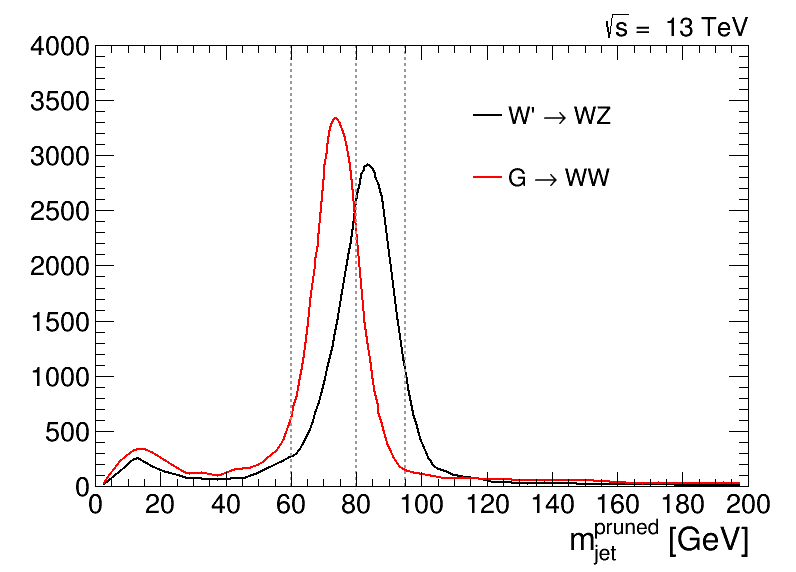
\includegraphics[width=0.7\textwidth]{\cheight/WVanalysis/prunedmass-discriminant-M1000.png}
 \caption{Pruned jet mass distributions of merged W-jets and merged Z-jets expected in G$\rightarrow$WW$\rightarrow l\nu qq$ and W'$\rightarrow$WZ$\rightarrow l\nu qq$ signals, respectively. The optimal separation point between the two distributions is shown together with the signal region boundaries.}
 \label{fig:WZcategories}
 \end{figure}
 
\begin{figure}[htbp]
 \centering
 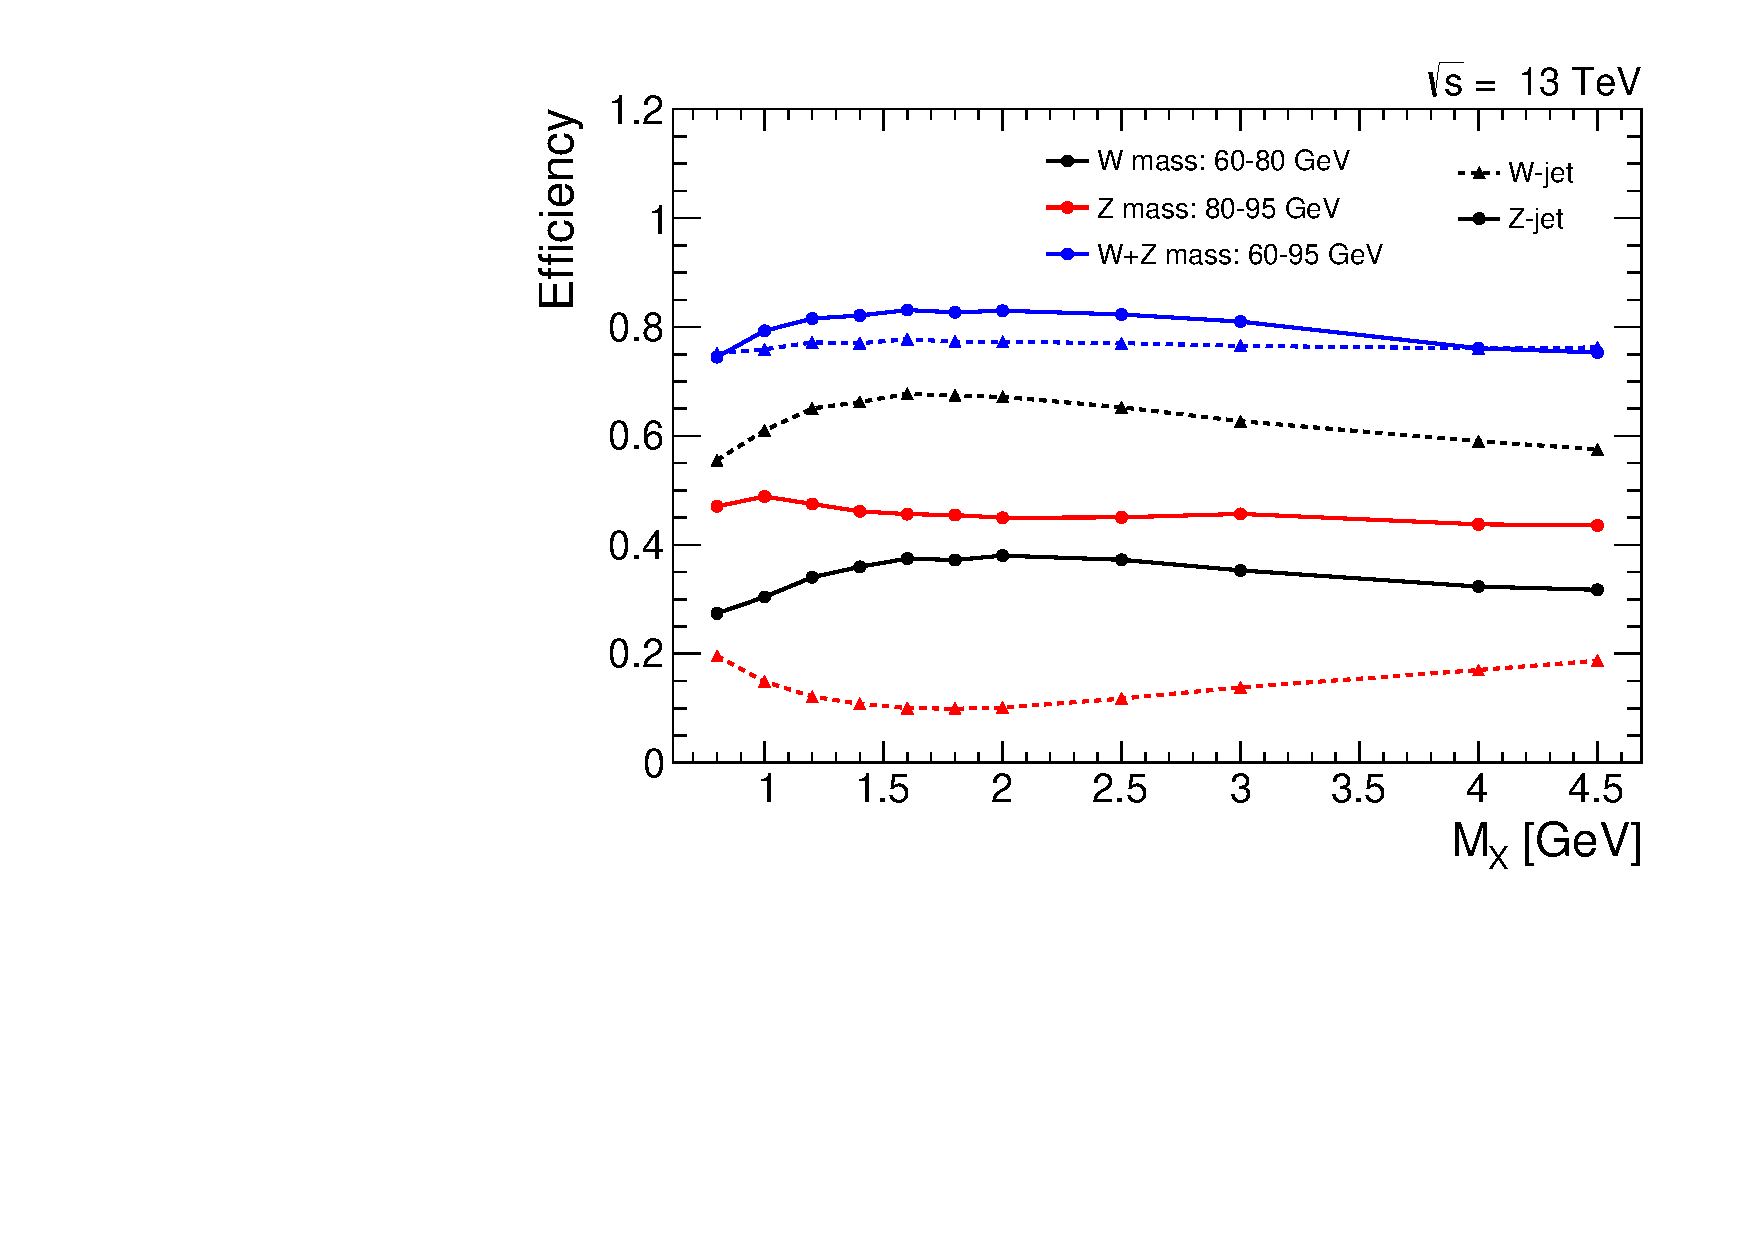
\includegraphics[width=0.7\textwidth]{\cheight/WVanalysis/prunedmass-eff.pdf}
 \caption{Efficiencies of a W-jet signal (G$\rightarrow$WW) (dashed lines) and of a Z-jet signal (W'$\rightarrow$WZ) (solid lines) as a function of the resonance mass for different pruned jet mass windows: W-mass category (black), Z-mass category (red) and default single mass category (blue).}
 \label{fig:massCategories_efficiency}
 \end{figure}
  
  \begin{figure}[htbp]
 \centering
 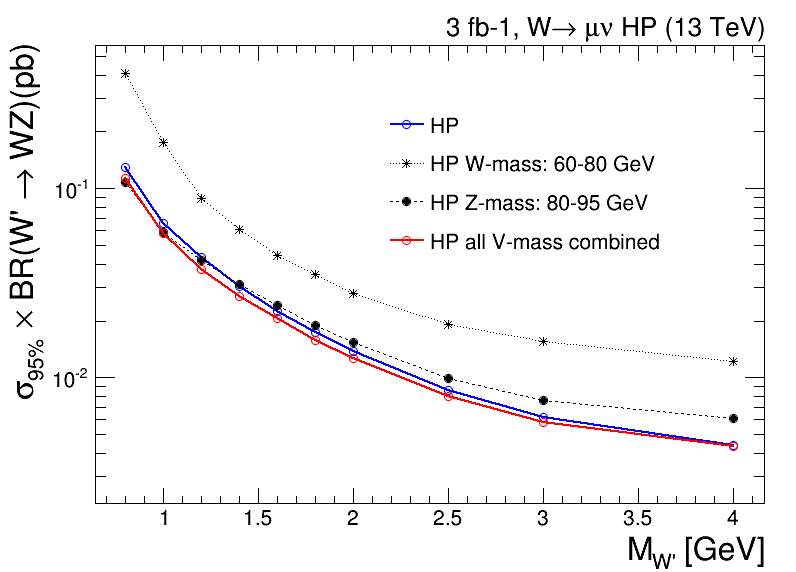
\includegraphics[width=0.48\textwidth]{\cheight/WVanalysis/compare-HP-HPV-Wprime.png}
  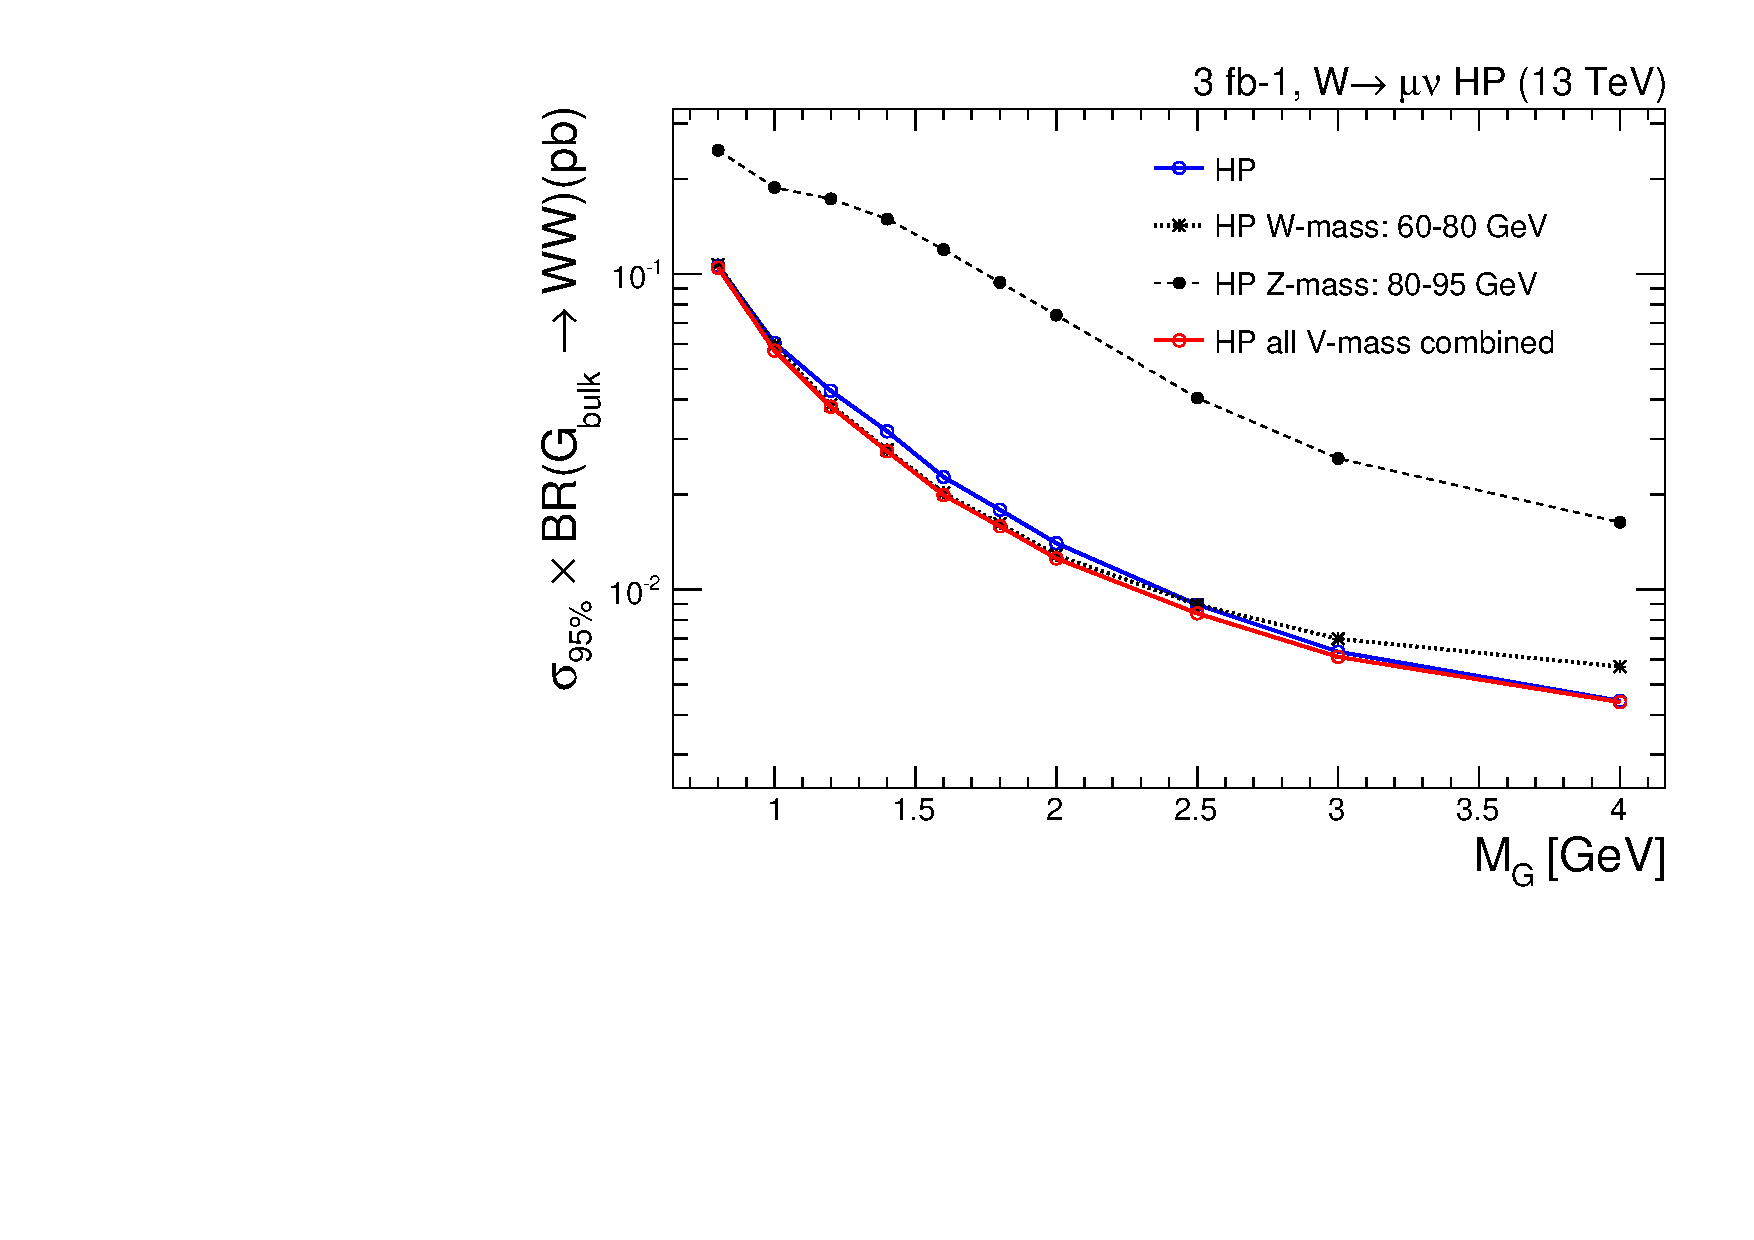
\includegraphics[width=0.48\textwidth]{\cheight/WVanalysis/compare-HP-HPV-BulkG.pdf} 
 \caption{Expected 95\% CL upper limits on the production cross section of a W' signal multiplied by the branching fraction of W'$\rightarrow$WZ as function of the resonance mass for the different mass categories for events passing the high-purity $\tau_{21}$ selections. Expected 95\% CL upper limits on the production cross section of a Graviton signal multiplied by the branching fraction of G$\rightarrow$WW as function of the resonance mass for the different mass categories for events passing the high-purity $\tau_{21}$ selections.}
 \label{fig:massCategories_limitsWp}
 \end{figure}

\begin{figure}[htbp]
 \centering
 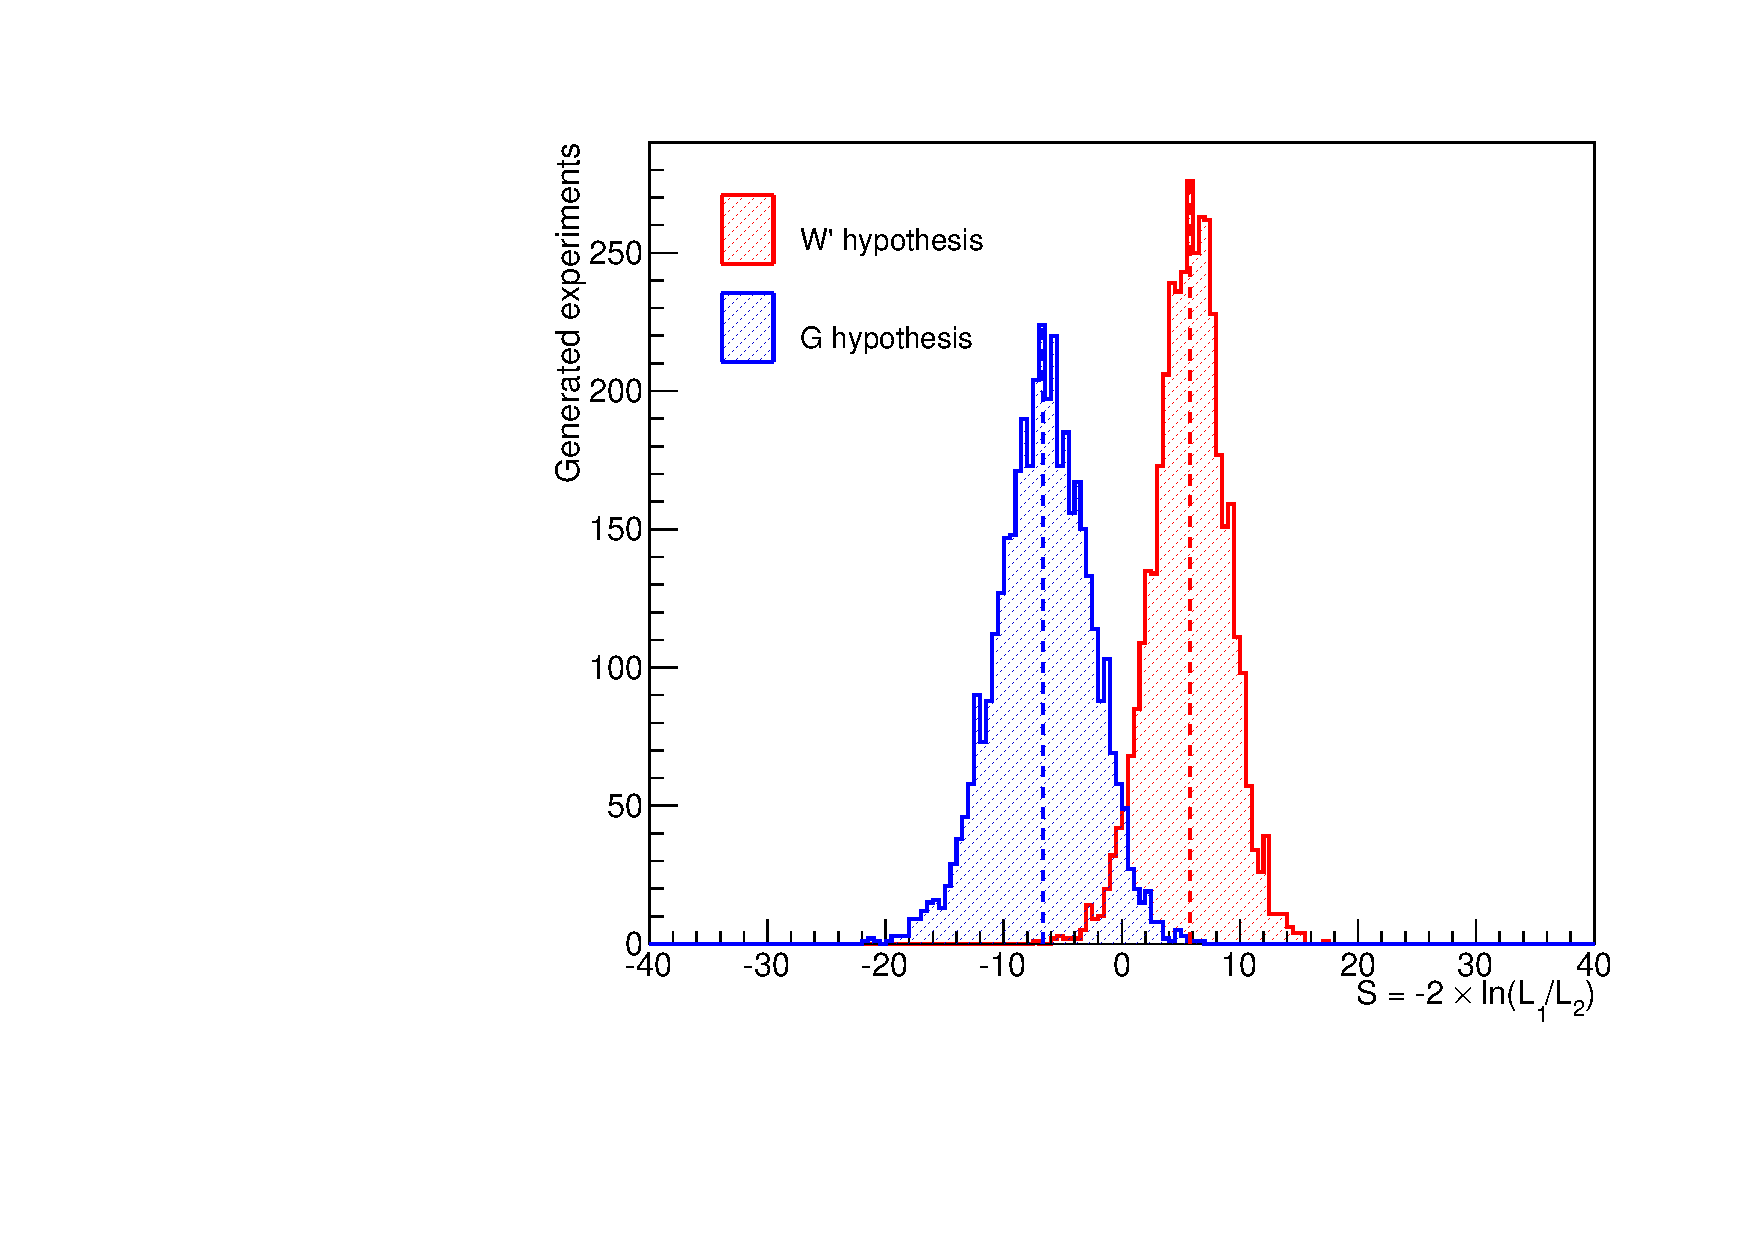
\includegraphics[width=0.7\textwidth]{\cheight/WVanalysis/sig_sep.pdf}
 \caption{Distribution of the test statistic $q = -2ln(L_{G}/L_{W'})$ of the Graviton signal hypothesis (blue) tested against the W' signal hypothesis (red). }
 \label{fig:signalsep}
 \end{figure}
 
 %%%%%% 
\subsection{Final selection and control plots}

\begin{table}[htb]
\footnotesize
\begin{center}
\caption{Summary of the VW channel final selection.}
\label{tab:cutsummaryWV}
\begin{tabular}{lcc}
\hline %%% Don't  you love the fact that we don't have the booktabs package? ^^
\multicolumn{1}{c}{\textbf{Selection}} & \textbf{Value} & \textbf{Comments}\\
\hline
\multicolumn{1}{c}{\texttt{Tight} Lepton selection}\\
\cline{1-1}
Electron $\PT$ & $\PT > 120 \GeV$    & \\
Muon $\PT$ & $\PT > 53 \GeV$ & \\
Electron $\eta$ & $|\eta|_{\text{SC}} <2.5$ except [1.4442, 1.566] range & Avoid the ECAL gap.\\
Muon $\eta$  & $|\eta|<2.1$  & \\
\hline
\multicolumn{1}{c}{\texttt{Loose} Lepton selection}\\
\cline{1-1}
Electron $\PT$ & $\PT > 35 \GeV$    & \\
Muon $\PT$ & $\PT > 20 \GeV$ & \\
Electron $\eta$ & $|\eta|_{\text{SC}} <2.5$ except [1.4442, 1.566] range & Avoid the ECAL gap.\\
Muon $\eta$  & $|\eta|<2.4$  & \\
\hline
\multicolumn{1}{c}{AK8 jet selections}\\
\cline{1-1}
Jet $\PT$ &  $\PT >200~\GeV$ & Used for hadronic \\
Jet $\eta$  & $|\eta|<2.4$ & W reconstruction \\
\hline
\multicolumn{1}{c}{AK4 jet selections}\\
\cline{1-1}
Jet $\PT$ &  $\PT >30~\GeV$ & Used for b-tag \\
Jet $\eta$  & $|\eta|<2.4$ & jet selection\\
\hline
\multicolumn{1}{c}{\ETmiss selections}\\
\cline{1-1}
\ETmiss (electron ch.) &  \ETmiss$>80~\GeV$ & \\
\ETmiss (muon ch.) & \ETmiss$>40~\GeV$ & \\
\hline
\multicolumn{1}{c}{Boson selections}\\
\cline{1-1}
Pruned jet mass (signal)        & $ 65 < m_{jet}^{pruned} < 105 \GeV$ &  \\
Pruned jet mass (low-mass sideband)       & $ 40 < m_{jet}^{pruned} < 65 \GeV$ & \\
Pruned jet mass (high-mass sideband)     & $ 105 < m_{jet}^{pruned} < 135 \GeV$ & \\
Leptonic W $\PT$      &  $\PT > 200 \GeV$     & \\
Hadronic W $\PT$      &  $\PT > 200 \GeV$     & \\
Back-to-back topology & $\Delta R (\ell , W_{had}) > \pi/2$ $\,$ , $\,$  $\Delta \phi (W_{had} , \mbox{\ETmiss})>2$ & \\ 
                      & $\Delta \phi (W_{had} , W_{lep})>2$ & \\
\hline
\multicolumn{1}{c}{Veto}\\
\cline{1-1}
Number of \texttt{loose} electrons & 0    & in addition to \texttt{tight} lepton \\
Number of \texttt{loose} muons & 0    & in addition to \texttt{tight} lepton \\
Number of b-tagged jets           & 0    & PF iCSV medium working point \\
\hline
\multicolumn{1}{c}{Diboson selections}\\
\cline{1-1}
2- to 1-subjettiness ratio (high purity) & $\tau_{21} < 0.60$                & \\
2- to 1-subjettiness ratio (low purity) & $0.60 \leq \tau_{21} < 0.75$ &\\
\hline						       
\end{tabular}
\end{center}
\end{table}

 \begin{figure}[htbp]
 \centering
 \begin{tabular}{cc}
 \includegraphics[width=0.45\textwidth]{\cheight/WVanalysis/ControlPlots_WJetsCR/mu/nPV_0}
 \includegraphics[width=0.45\textwidth]{\cheight/WVanalysis/ControlPlots_WJetsCR/el/nPV_0}\\
 \includegraphics[width=0.45\textwidth]{\cheight/WVanalysis/ControlPlots_WJetsCR/mu/l_pt_0}
 \includegraphics[width=0.45\textwidth]{\cheight/WVanalysis/ControlPlots_WJetsCR/el/l_pt_0}\\
 \includegraphics[width=0.45\textwidth]{\cheight/WVanalysis/ControlPlots_WJetsCR/mu/l_eta_0}
 \includegraphics[width=0.45\textwidth]{\cheight/WVanalysis/ControlPlots_WJetsCR/el/l_eta_0}\\
 \end{tabular}
 \caption{Comparison plots between data and MC for different observables, in the jet mass sideband.
 From top to bottom: number of primary vertices, lepton \PT{}, lepton $\eta$. 
 Left: muon channel, right: electron channel. }
 \label{fig:Wjets_controlPlots_1}
 \end{figure}

 \begin{figure}[htbp]
 \centering
 \begin{tabular}{cc}
 \includegraphics[width=0.45\textwidth]{\cheight/WVanalysis/ControlPlots_WJetsCR/mu/pfMET_0}
 \includegraphics[width=0.45\textwidth]{\cheight/WVanalysis/ControlPlots_WJetsCR/el/pfMET_0}\\
 \includegraphics[width=0.45\textwidth]{\cheight/WVanalysis/ControlPlots_WJetsCR/mu/v_pt_0}
 \includegraphics[width=0.45\textwidth]{\cheight/WVanalysis/ControlPlots_WJetsCR/el/v_pt_0}\\
 \includegraphics[width=0.45\textwidth]{\cheight/WVanalysis/ControlPlots_WJetsCR/mu/v_mt_0}
 \includegraphics[width=0.45\textwidth]{\cheight/WVanalysis/ControlPlots_WJetsCR/el/v_mt_0}\\
 \end{tabular}
 \caption{Comparison plots between data and MC for different observables, in the jet mass sideband.
 From top to bottom: \MET{}, leptonic W \PT{}, transverse mass of the leptonic W. 
 Left: muon channel, right: electron channel. }
 \label{fig:Wjets_controlPlots_2}
 \end{figure}

 \begin{figure}[htbp]
 \centering
 \begin{tabular}{cc}
 \includegraphics[width=0.45\textwidth]{\cheight/WVanalysis/ControlPlots_WJetsCR/mu/ungroomed_jet_pt_0}
 \includegraphics[width=0.45\textwidth]{\cheight/WVanalysis/ControlPlots_WJetsCR/el/ungroomed_jet_pt_0}\\
 \includegraphics[width=0.45\textwidth]{\cheight/WVanalysis/ControlPlots_WJetsCR/mu/ungroomed_jet_eta_0}
 \includegraphics[width=0.45\textwidth]{\cheight/WVanalysis/ControlPlots_WJetsCR/el/ungroomed_jet_eta_0}\\
 \end{tabular}
 \caption{Comparison plots between data and MC for different observables, in the jet mass sideband.
 Top: \PT{} of the leading AK8 jet. Bottom: $\eta$ of the leading AK8 jet. 
 Left: muon channel, right: electron channel. }
 \label{fig:Wjets_controlPlots_3}
 \end{figure}

 \begin{figure}[htbp]
 \centering
 \begin{tabular}{cc}
 \includegraphics[width=0.45\textwidth]{\cheight/WVanalysis/ControlPlots_WJetsCR/mu/jet_mass_pr_0}
 \includegraphics[width=0.45\textwidth]{\cheight/WVanalysis/ControlPlots_WJetsCR/el/jet_mass_pr_0}\\
 \includegraphics[width=0.45\textwidth]{\cheight/WVanalysis/ControlPlots_WJetsCR/mu/jet_tau2tau1_0}
 \includegraphics[width=0.45\textwidth]{\cheight/WVanalysis/ControlPlots_WJetsCR/el/jet_tau2tau1_0}\\
 \end{tabular}
 \caption{Comparison plots between data and MC for different observables, in the jet mass sideband.
 Top: pruned jet mass. Bottom: N-subjettiness. 
 Left: muon channel, right: electron channel. }
 \label{fig:Wjets_controlPlots_4}
 \end{figure}